%% LyX 1.6.7 created this file.  For more info, see http://www.lyx.org/.
%% Do not edit unless you really know what you are doing.
\documentclass[english]{article}
\usepackage[T1]{fontenc}
\usepackage[latin9]{inputenc}
\usepackage{amstext}
\usepackage{graphicx}
\usepackage{esint}
\usepackage{babel}

\begin{document}

\section{Introduction}

The purpose of this document is to clearly describe what my thesis
is trying to do. Much of it will be able to go directly into the thesis,
but I'm writing it in a more informal mode, since doing so is helping
me to actually get this stuff written down, and I'm hoping it will
also help with understanding what I'm trying to do, and allow constructive
criticism. I will describe some of the nuts and bolts of micro-economics,
as well as covering broader questions. 


\subsection{The overall aim of the thesis}

The most important aim is this: to take some good elements from 'standard'
micro-economics and some good elements from agent-based modelling,
and use them to ask the most basic question about geographical economics:
how do places form? What are the 'best parts' the thesis works with,
and what is deficient from each method?
\begin{itemize}
\item Neoclassical economics has an excellent generic framework for describing
the structure of the economy, able to describe the relationship between
all goods. In principle, this means the entire economy can be described
within that framework, and questions asked of a `general' nature -
where `general' in this case is the whole-world counterpart to `partial'
analyses that only examine a subset of that whole.
\item Agent-based modelling is able to investigate what happens when many
heterogenous actors interact. A main premise of this thesis is that
space presupposes heterogeneity because actors face differenet costs
depending on location. So ABM should, in theory, be a useful tool
for investigating its effects.
\item The deficiencies of each theory are slightly different: economics
has difficulty with heterogeneity - and so perhaps ABM can be useful.
The problems with ABM stem from its relationship to `complexity'.
One result of this, for example, has been that - as far as I can tell
- there has been little interest in using the sort of generic framework
that micro-economics provides for asking 'general' questions about
location. This may also be because one of the central methods of economics
- the abstract model - has been misunderstood, and is generally derided
as unrealistic outside of economics. This is discussed more below.
\end{itemize}

\section{Market structure and space}

There are three broad categories of favoured market structure in analytic
economics: perfect competition, monopoly and monopolistic competition.
Why `favoured'? Each of these are analytically tractable. Perfect
competition models can assume that actors all face the same prices,
and can have no influence over them - they are too small compared
to the extent of the market. Monopoly models can say how a single
firm should set its prices to maximise revenue, when faced with a
particular demand curve - and because there is only one firm, there
are no strategic considerations. 

Outside of the two poles of perfect competition and monopoly, the
monopolistic competition model \textbackslash{}gls\{monocomp\} first
published by \textbackslash{}citeauthor\{dixit\_monopolistic\_1977\}
in 1977 is by far the most popular approach to market structure in
spatial settings. The approach itself is explained in-depth below,
but before that it is important to grasp why the model was needed:
it is impossible to combine perfect competition models with space.
Why not? There are two related reasons. First: perfectly competitive
models must work with linear output - no economies of scale (or `increasing
returns') are allowed. To see why, consider a (rather artificial)
situation where many firms have linear output, but one firm, producing
the same good, is able to utilise economies of scale. They can thus
produce each unit more cheaply than their competitors - and so this
is no longer a perfect competition situation. A single price can no
longer be assumed, nor can one say that no actor can influence price.
In this case, that one firm immediately gains monopoly power. Second:
it is impossible to include space in a model \emph{without} increasing
returns - and so space and perfect competition models cannot be combined.
Again, why not? Starrett (1978) is credited with first making this
point formally. As Fujita and Thisse describe it -
\begin{quote}
``The essential question is whether the competitive price mechanism
is able to explain the endogenous formation of economic agglomerations.
To check the ability of a spatial model to do so, the best approach
is to consider the case of a homogenous space in which economic agents
are free to choose their locations... Starrett has shown that if space
is homogenous and transport costly, then... the economy degenerates
into separate single-location groups of agents with all trades taking
place within, rather than between, groups. Consequently, the perfectly
competitive price mechanism alone is unable to deal simultaneously
with cities and trade.'' (Fujita Thisse book p.13-14)
\end{quote}
To put it another way: if an actor is able to produce `in their own
backyard', why would they choose to trade or collaborate? Any gain
they would receive can never outweigh transport costs, if output in
linear. However, with increasing returns introduced to the picture,
the minimum conditions for spatial economic activity now exist. This
`minimum condition for agglomeration' is investigated in an agent
context through the 'backyard' series of models in this thesis. It
is worth noting that, historically, 'backyard' production of various
sorts has been a commonplace. Sheffield cutlers, for example, worked
in this way, with many homes having their own mini-forges. {[}citation{]} 

In the discipline of economics, up until the publication of the Dixit/Stiglitz
model, arguments about space in economic models had not moved on much
from the 1940s and 1950s. As Krugman points out -
\begin{quote}
``... in the late 1980s mainsteam economists were almost literally
oblivious to the fact that economies aren't dimensionless points in
space.'' (Krugman, middle aged, p.1)
\end{quote}
This was at least in part because of earlier debates where economists
had parted ways with a nascent regional science: the former insisted
that perfect competition models could include space implicitly as
part of their cost structure; the latter argued that was nonsense.
(Isard is one such, and it is interesting to note that he also seems
to have little time for GE-style use of transport costs: ``... it
is as unjustifiable and inadequate to lump transport costs into one
category along with all trade resistances in the theory of trade,
as it is to treat them as implicit production costs in the theory
of production.'' (Isard 56? p.478) ) After Krugman's reinterpretation
of Dixit-Stiglitz in a spatial context, monopolistic competition gained
two vital qualities appealling to mainstream economists: tractability
and determinacy..


\section{Utility}

At its simplest, utility is a very effective way of describing when
an economic actor is better or worse off. It can abstract away from
any details about the nature of `better off' in any psychological
sense. This is a strength of utility theory, though it is often portrayed
as a weakness. Later, these arguments will be examined in more depth,
since they impact on the way that agent modellers have chosen to approach
economics. The task here is to explain the forms of utility that will
be used in this thesis.

The simplest form of utility function to be used here is the Cobb
Douglas. A consumer gets utility from two goods, labelled $F$ and
\textbf{$M$.} (For consistency, the variable names here are the same
as those used later when discussing geographical economics.)

\begin{equation}
U=F^{a}M^{b}\label{eq:-1}\end{equation}


The sum of $a$ and \textbf{$b$} control returns to scale. Summing
the exponents to one gives constant returns to scale, whereas if $a+b>1$,
the function has increasing returns. Most commonly it is assumed that
$a+b=1$. For this, an equivalent function can be used:

\begin{equation}
U=F^{\delta}M{}^{1-\delta}(0<\delta<1)\label{eq:-3}\end{equation}


This Cobb Douglas is particularly popular because of the convenient
relationship that exists between a consumer's budget and the optimal
mix of $F$ and \textbf{$M$. }Let $Y$ be the consumer's budget.
Assuming the cost of both $F$ and \textbf{$M$} is unity (they both
have a price of one), total consumption cannot be more than the budget: 

\begin{equation}
F+M=Y\label{eq:-2}\end{equation}


What, then, is the optimal mix of the two goods for the consumer?
The answer can be guessed from simply graphing the function (see figure\textasciitilde{}\textbackslash{}ref\{fig:cobbdouglasgraph1\}).
More formally, maximising \ref{eq:-3} with the budget constraint
\ref{eq:-2} gives -

\[
F=\delta Y\]


\[
M=1-\delta Y\]


(See Varian pp.100, Chiang and Wainwright pp.386 and section ??? in
appendix for the derivation.) So, for example, if $\delta=0.5$ and
the consumer's budget $Y=10$, their utility-maximising mix would
be five for each good. These preferences would also be homothetic
- if the budget changed, the proportionate mix of optimal goods would
remain the same. 

The Cobb Douglas exhibits, in the simplest way possible, a basic feature
used by \textbackslash{}gls\{ge\}: 'love of variety' - a mix of the
two goods is preferable to either good alone. (The optimal mix here
defined with $\delta$, which can be referred to as the 'share parameter'.)
Figure \ref{cobbdouglas2}illustrates this point: the contour lines
indicate isoquants: lines of equal utility, where a consumer would
be indifferent between the mix of $F$ and $M$, if their budget didn't
matter. However, it does: so their optimal choice is a line through
all possible budgets.

Love of variety is such a key concept it is worth spending a few moments
on the intuition of what it represents. Two identical meals in a row
for lunch and dinner, each consisting of a homogenous gloop, is likely
to be less satisfying than a good lunch and a three course dinner.
At a very different scale, it may also be true that consumers prefer
- in aggregate - a choice between four models of car than two, though
in total they may buy the same number of cars. 

While the Cobb Douglas does have this dynamic, it is the 'constant
elasticity of substitution' (CES) function that can best represent
it. The CES function can control `love of variety' with a single parameter.
The `desirability of variety' is central to Dixit and Stiglitz's 1977
paper on monopolistic competition. They note that many theorists have
attacked the problem, often through `product space' approaches, which
they find lack generality. Instead, they propose a much simpler solution
- using a function able to reflect that:
\begin{quote}
``... a consumer who is indifferent between the quantites $(1,0)$
and $(0,1)$ of two commodities prefers the mix ($\frac{1}{2},\frac{1}{2}$)
to either extreme.'' (dixit stiglitz 77 p.297)
\end{quote}
It is easiest to see how this works in a simple two-good function
that looks like Dixit and Stiglitz's example, before moving on to
the n-good case. Consider a consumer with the utility function:

\begin{equation}
U=\left[F^{\rho}+M^{\rho}\right]^{1/\rho}\label{eq:-4}\end{equation}


The first thing to note is that, if we suppose $M=0$, and only $F$
has a positive value, then $U=(F^{\rho})^{1/\rho}$. This is always
just $U=F$, regardless of the value of $\rho$. If both goods have
positive values, and$\rho=1$, this reduces to $U=F+M$ and utility
is also entirely linear. But for $0<\rho<1$, the consumer is better
off with a mix of the two goods as $\rho\rightarrow0$. So, for example,
let $F=4$ and $M=4$. If $\rho=1,$this means utility is just 8.
If $\rho=\frac{1}{2}$, however, $F$ and $M$ both become $2$. So
utility is then just $(2+2)^{2}$or 16 - double the linear result.
In effect, then, $\rho$is the love of variety. For values of $0<\rho<1$,
the two goods are imperfect substitutes. This can be seen if the function
is altered slightly to:

\begin{equation}
U=\left[\delta F^{\rho}+(1-\delta)M^{\rho}\right]^{1/\rho}\label{eq:-5}\end{equation}


Again, $\delta$ is a share parameter: the consumer must choose a
limited mix of the two goods. As figure ??? illustrates, a consumer
is best off with a perfect mix of the two, rather than either extreme.
This is just a restatement of Dixit and Stiglitz's original point;
however the simple principle illustrated here holds for all other
versions of the CES. The Cobb Douglas is a special case of the CES
where $\rho=0$.

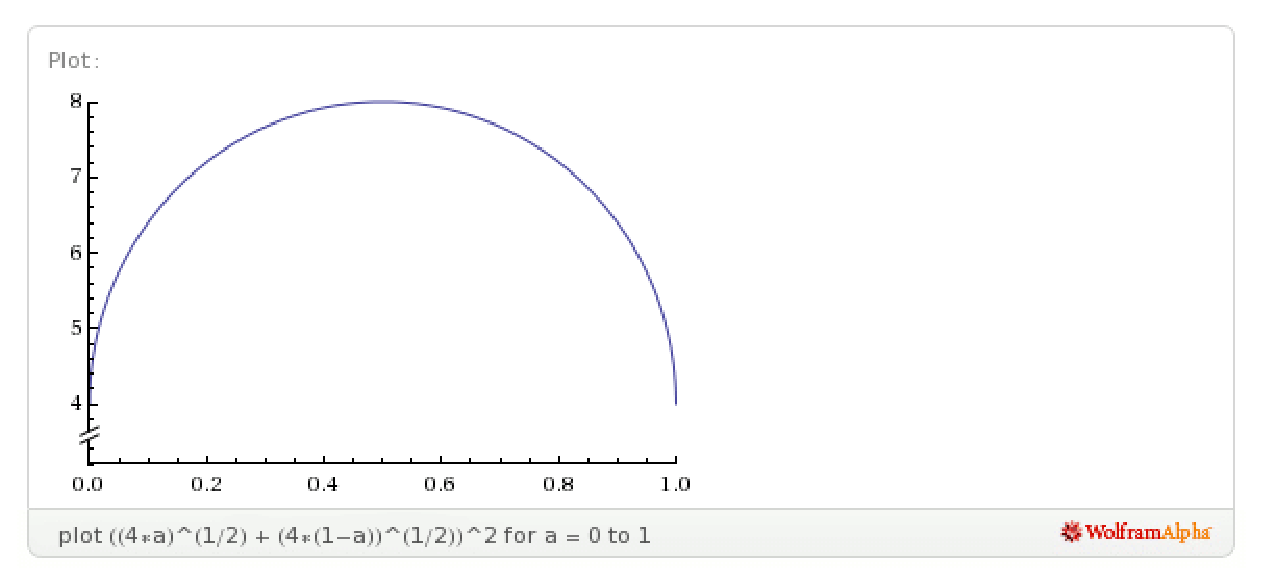
\includegraphics[width=9cm]{images/substitution}

The many-good CES comes in two varieties: discrete and continuous.
For the former - 

\begin{equation}
U=\left(\sum_{i=1}^{N}c_{i}^{\rho}\right)^{1/\rho}\label{eq:-6}\end{equation}


In this version, $c$ denotes the quantity of good $i$ and can -
in theory - be set individually, so that utility is dependent on the
sum of all goods. However, usually in geographical economics, consumption
of each good is symmetric: quantities for each are the same. Given
this, a continuous integral can also be used to describe utility:

\begin{equation}
U=\left[\int_{0}^{n}i^{\rho}di\right]^{1/\rho}\label{eq:-7}\end{equation}


This is used in Dixit and Stiglitz's formulation for monopolistic
competition (see also Fujta et al 1999 p.46), whereas the discret
version is used more in work related to the core model.


\subsection{An illustration: the CES function in trade theory}


\section{Production functions}

Both utility and firm production can be described using the same mathematical
tools, and often are. In the core theory, demand from actors is used
to imply the level of production directly - so utility and production
functions are bound together.. This is doubtless all very familiar
to economists - it's one of many things that I've found highly perplexing
as I've been trying to understand how the economics works.

What are the factors that go into production, and how are they combined?
In analytic economics, it is most often the job of a production function
to turn factor inputs into an output. The kind of production function
used in simple models tend themselves to be simple; generally, `tractable'
wins over `realistic': a black box approach where inputs are clearly
defined through an equation into some single output. 

Some particular reasons why simple production (and utility) models
are commonly used:
\begin{enumerate}
\item When optimised (with a Lagrange multiplier in the core model), they
produce easily useable results. 
\item They provide parameters that can easily be attributed to particular
real-world features, such as substitutability between factors.
\end{enumerate}
Probably easiest to look at some examples for this. 

Jane Jacobs' arguments in particular present problems for the straightforward
'black box' model. Where the point of those models is that an in-out
relationship can be defined - and only altered through some technological
change - Jacobs' description of production paints a picture of economic
actors stumbling upon new combinations of goods in a way very reminiscent
of evolution. 

Perhaps the most challenging productive factor to theorise is knowledge.
An example from Krugman illustrates the sort of interactions that
can take place. He argues that as energy became cheaper and more accessible,
it could substitute for skilled labour. The result was a replacement
of that labour by cheap energy sources - and an increase in the footloose
mobility of workers, because pools of local skilled labour were now
less necessary. 


\section{Criticism}

The kind of production and utility functions described get plenty
of criticism, aimed in one way or another at their intrinsic lack
of realism. Ecological economics, for example, sees in the Cobb Douglas
function a 'Garden of Eden' world (GR quoted in Daly) where natural
resources are optional. Daly sums this up nicely, if somewhat loquaciously.
He responds to Solow's line that ``If it is very easy to substitute
other factors for natural resources, then there is in principle no
`problem'. The world can, in effect, get along without natural resources''
(quote in Daly, Georgescu-blah p.261).

Daly responds that economists seem to believe in ``making a cake with
only the cook and his kitchen. We do not need flour, eggs, sugar,
etc., nor electricity or natural gas, nor even firewood. If we want
a bigger cake, the cook simply stirs faster in a bigger bowl and cooks
the empty bowl in a bigger oven that somehow heats itself.'' (ibid.)

More formally, he quotes Georgescu-Rosen's critique of the Solow-Stiglitz
production function - a Cobb Douglas with the addition of natural
resources:

\begin{equation}
Q=K^{a1}R^{a2}L^{a\text{3}}\label{eq:}\end{equation}


He points out this means that $R^{a2}=Q/K^{a1}L^{a3}$. So, holding
labour constant, one could get any quantity of output with as small
an amount of R, as long as R > 0 and K is large enough to compensate
for that tiny amount. 

Solow's reply to this highlights a recurring argument used to defend
the abstract nature of many economic models: critics are taking them
too literally, and not considering how the models are used. Solow
counters with:
\begin{quote}
``We were trying to think about an interesting and important question:
how much of a drag on future growth, or even on the sustainability
of current production, might be exercised by the limited availability
of natural resources and the inputs they provide? ... The role of
theory is to explore what logic and simple assumptions can tell us
about what data to look for and how to interpret them in connection
with the question asked.'' (solow p.267/8)
\end{quote}
Solow goes on to point out that the argument should be about how substitutable
renewable and non-renewable resources are, given that the former are
likely to be highly capital-intensive. (Ibid.) He clearly does understand
the issues; what the critics seem to have done is mistake the economists'
models for their actual understanding of the world, rather than tools
that aid that understanding. Krugman makes much the same kind of plea.
{[}insert details here!{]} A clear example of this also comes from
Krugman's work on international trade, discussed above, and cannot
be put better than Krugman himself does in the abstract to his original
1979 paper: 
\begin{quotation}
``... trade, and gains from trade, will occur, even between countries
with identical tastes, technology, and factor endowments.'' (Krugman
1979 p.469)
\end{quotation}
Or rather, they will occur in the model that Krugman presents. The
model itself cannot guarantee the real world contains the same dynamic;
the point is to show that such a dynamic is \emph{possible,} given
a particular set of assumptions. 

x

While Solow and Krugman are in large part correct, there are problems
with their case. Most fundamentally, there is a large gap between,
say, Krugman's stated awareness of a model's ``silly assumptions''
and the uses to which those models are now being put in policy circles. 

Pursuit of that argument, however, is beyond the scope of the thesis.
The more important issue at hand is this: there are implications for
agent modelling. How so? It comes back to Daly's claim that standard
economic functions offer only ``a technical production recipe that
contradicts both the first and second laws of thermodynamics, as well
as best practice in cooking.'' (p.262) Consider an agent model of
production that has aspirations to examine the complex morphology
of linkages seen in reality - Jane Jacobs' `tangled bank'. Agent models
are almost always explicitly time-driven; computer cycles are synonymous
with timesteps and iteration is central. In such a world, what moves
between economic linkages each timestep, if not actual resources?
Certainly, many exchanges can be service-related, but in a time-driven
model it becomes much harder to conceive of resources in an abstract
way. Instead, a more Weberian image presents itself as the most likely:
resources with weights, combined to produce other resources with weights.
\end{document}
